\documentclass[tikz, crop, border=5pt]{standalone}
\usetikzlibrary{positioning,backgrounds,fit}

\usepackage{fontspec}
\usepackage{xeCJK}

\setmainfont{NotoSans}[
    Extension      = .ttf,
    UprightFont    = *-Regular,
    BoldFont       = *-Bold,
    ItalicFont     = *-Italic,
    BoldItalicFont = *-BoldItalic
]

\usepackage{color}
\definecolor{red}{RGB}{255,59,48}
\definecolor{yellow}{RGB}{255,204,0}
\definecolor{grey}{RGB}{180,180,182}

% 添加热图所需的包和设置
\usepackage{pgfplots}
\pgfplotsset{
    compat=1.18,
    every axis/.append style={
        enlargelimits=false,
        axis line style={grey, thick},
        axis on top,
        tick style={draw=none},
        xtick={},
        xticklabels={},
        x tick label style={font=\footnotesize},
        extra x tick style={
            grid=major, grid style={grey, thick},
        },
        ytick=data,
        y tick label style={
            font=\normalsize,
            align=center,
        },
        extra y tick labels={},
        extra y tick style={
            grid=major, grid style={grey, thick},
        },
        colormap={mymap}{
            color(0)=(white)
            color(0.05)=(yellow!50)
            color(0.2)=(yellow)
            color(0.4)=(yellow!70!red)
            color(0.6)=(yellow!50!red)
            color(0.8)=(yellow!25!red)
            color(1)=(red)
        },
        colorbar,
        colorbar style={
            width=2mm,
            height=1cm,
            ytick={0,0.5,1},
            y tick label style={
                font=\footnotesize,
                align=left,
            },
        },
        point meta min=0,
        point meta max=1,
    },
    every colorbar/.append style={
        tick style={draw=none},
        axis line style={draw=none},
        at={(current axis.south east)},
        yshift=+0.5cm,
        anchor=west,
        label style={/pgf/number format/assume math mode=true},
        tick label style={/pgf/number format/assume math mode=true},
    },
}

\begin{document}

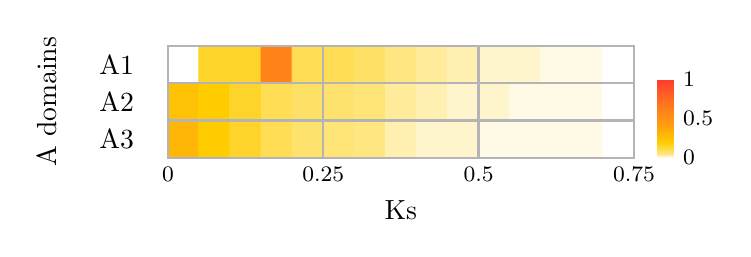
\begin{tikzpicture}
    \begin{axis}[%
%AXIS_BEGIN%
        width=7.5cm,
        height=3cm,
        xlabel={Ks},
        ylabel={A domains},
        extra x ticks={-0.5, 4.5, 9.5, 14.5},
        extra x tick labels={0, 0.25, 0.5, 0.75},
        yticklabels={A1, A2, A3},
        extra y ticks={-0.5, 0.5, 1.5, 2.5},
        y tick label style={
            text width=3em,
        },
%AXIS_END%
        ]
        \addplot[
            matrix plot,
            empty line=auto,
            % mesh/cols=15,
            point meta=explicit,
        ] table [meta=C] {
            x y  C
%TABLE_BEGIN%
            0 0  0
            1 0  0.15
            2 0  0.15
            3 0  0.60
            4 0  0.10
            5 0  0.10
            6 0  0.08
            7 0  0.05
            8 0  0.04
            9 0  0.03
            10 0  0.02
            11 0  0.02
            12 0  0.01
            13 0  0.01
            14 0  0

            0 1  0.25
            1 1  0.20
            2 1  0.15
            3 1  0.10
            4 1  0.08
            5 1  0.07
            6 1  0.06
            7 1  0.04
            8 1  0.03
            9 1  0.02
            10 1  0.02
            11 1  0.01
            12 1  0.01
            13 1  0.01
            14 1  0

            0 2  0.30
            1 2  0.20
            2 2  0.15
            3 2  0.10
            4 2  0.07
            5 2  0.06
            6 2  0.05
            7 2  0.03
            8 2  0.02
            9 2  0.02
            10 2  0.01
            11 2  0.01
            12 2  0.01
            13 2  0.01
            14 2  0
%TABLE_END%
        };
    \end{axis}
\end{tikzpicture}

\end{document}
